Since the beginnings of the 2000s knitting has encountered a steady rise in popularity. This might be due to the rise of the internet and social media, and the increasingly important role they play in the daily life. The older knitting generation is adapting the technology and switching over, and bringing knitting as a craft and hobby closer to the younger generations (\cite{lewis_rise_of_knitting}). Online communities like Ravelry\footnote{\url{http://www.ravelry.com/}} and Youtube\footnote{\url{https://www.youtube.com/}} teach the knitting enthusiasts knittings techniques and patterns of all kinds --- never has knitting knowledge been more accessible.

\begin{wrapfigure}{R}{0.5\textwidth}
    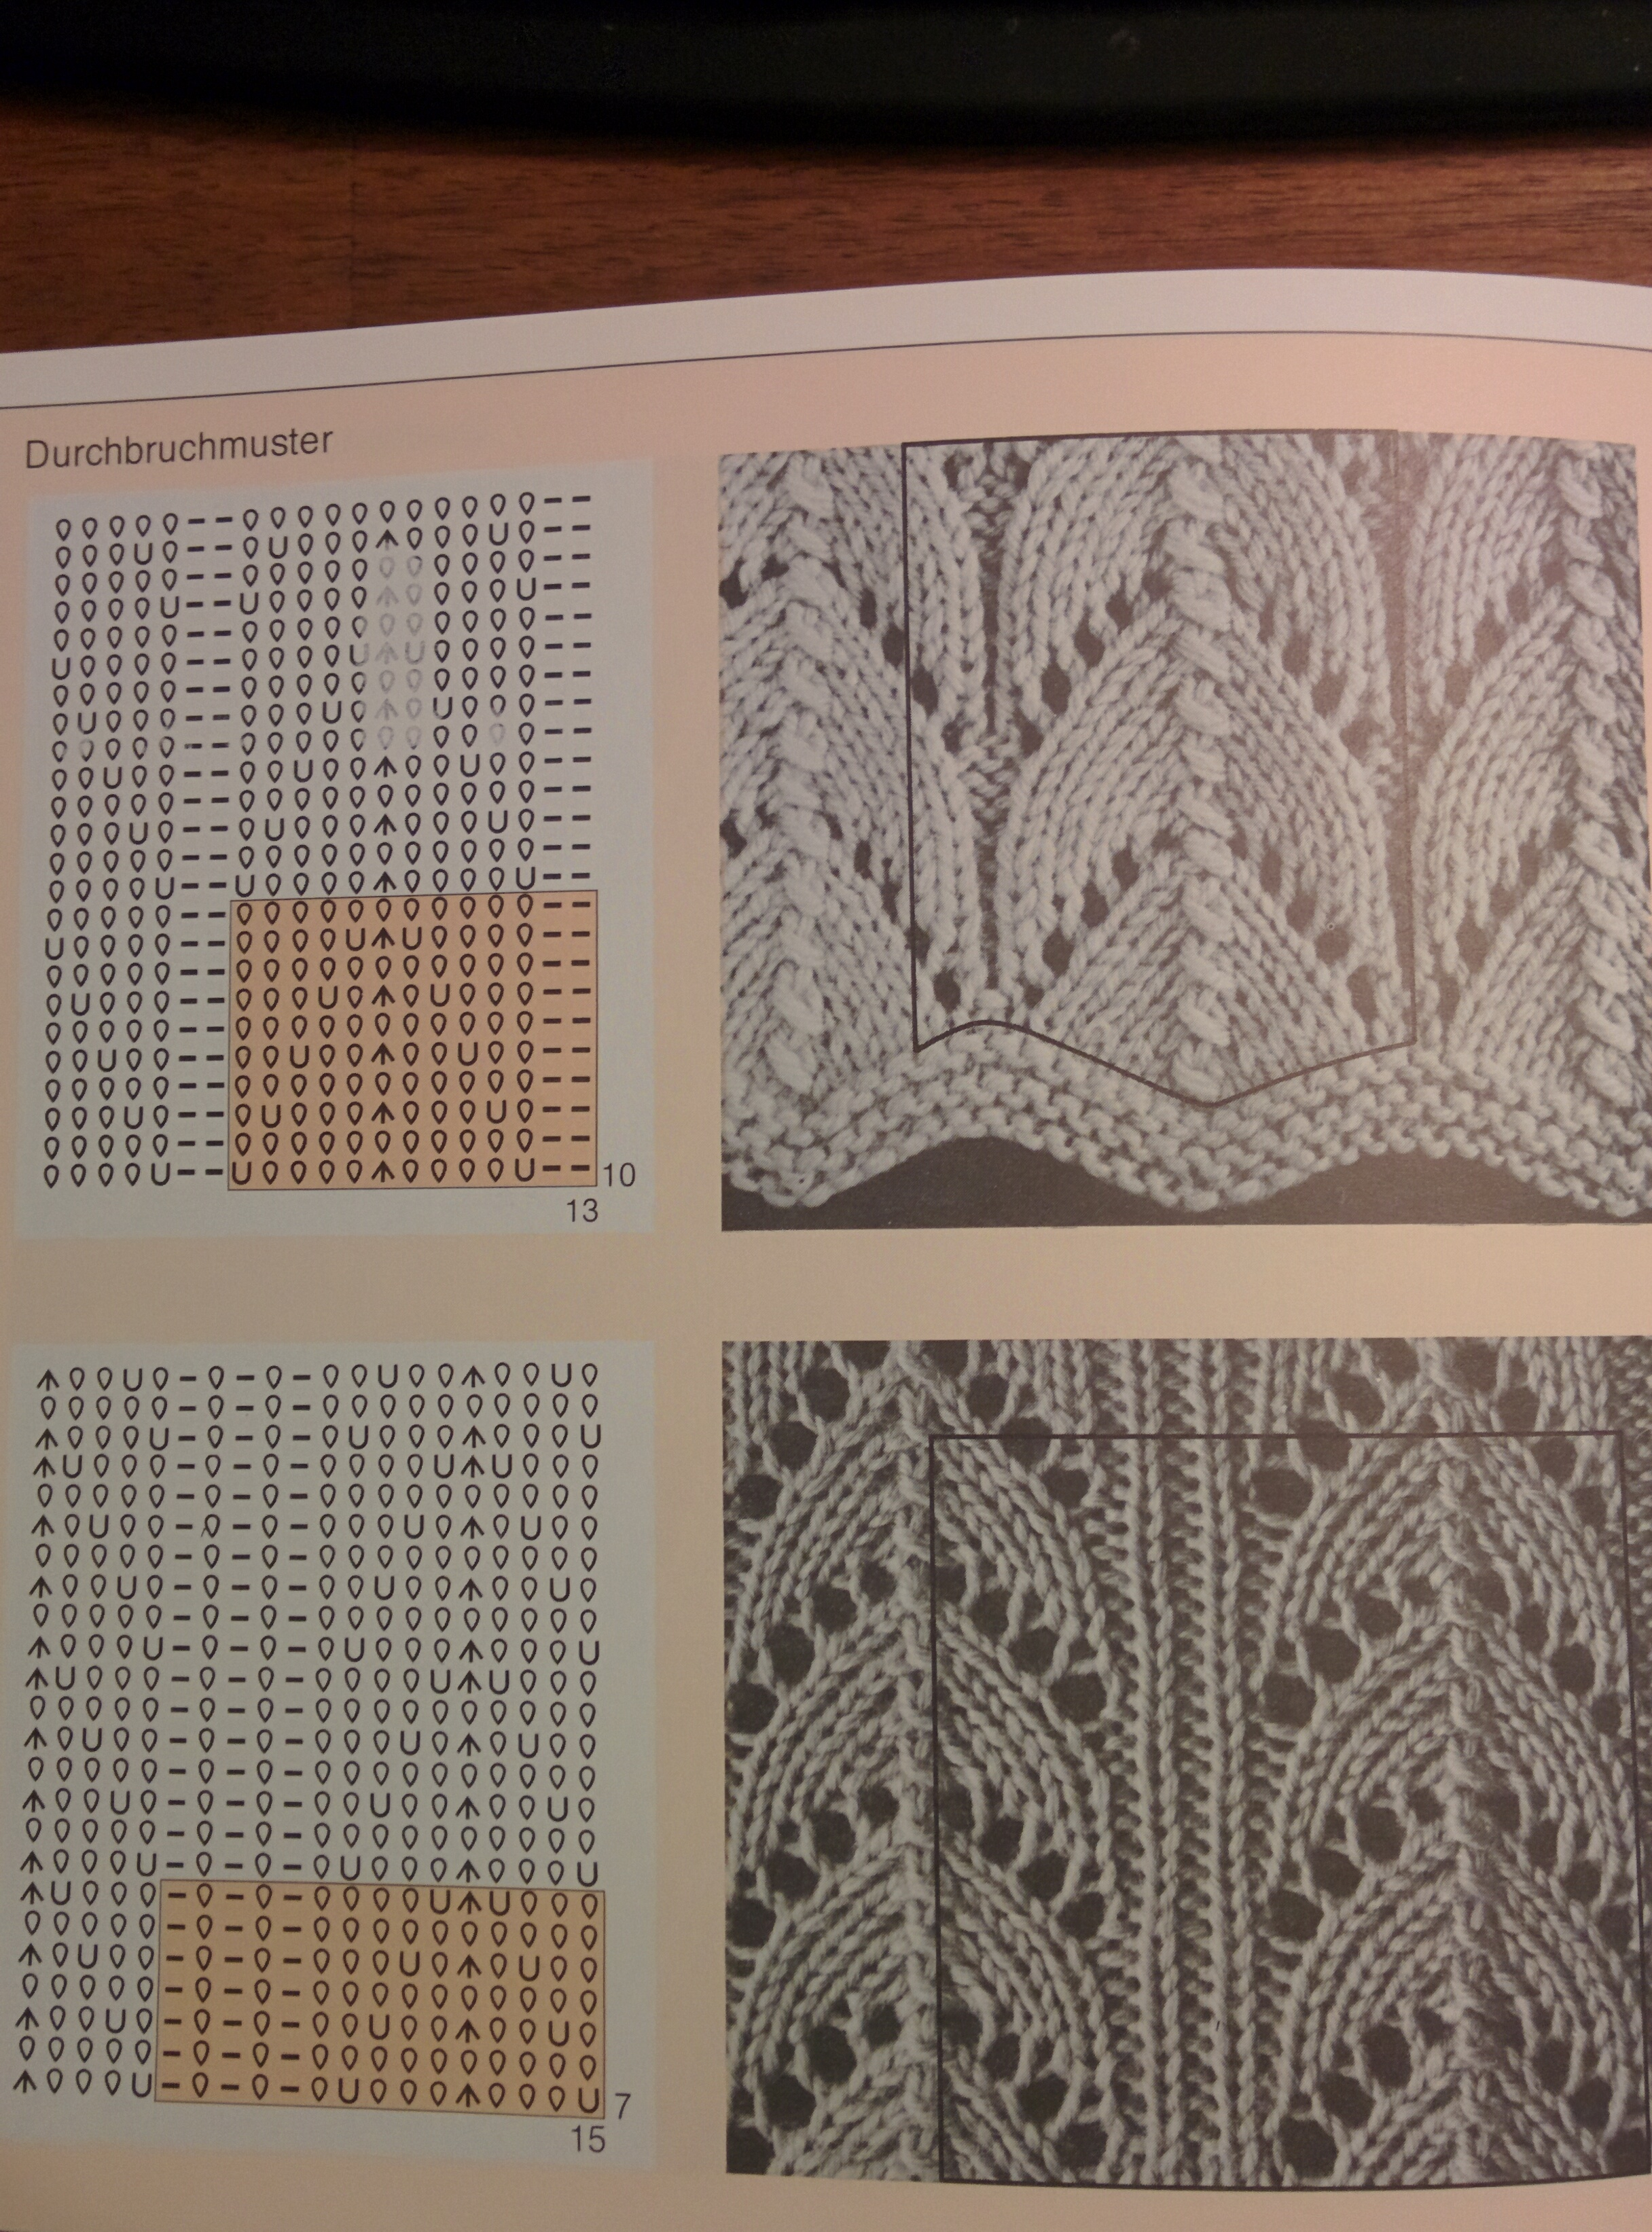
\includegraphics[width=1\linewidth]{images/knitting_pattern_chart_book.JPG}
   \caption[{Knitting patterns and their corresponding pattern charts \protect\newline{\small from \protect\cite[p142]{Natter1983}}}]{Knitting patterns and their corresponding pattern charts from \protect\cite[p142]{Natter1983}}
\end{wrapfigure}

Considering this it is all the more surprising that there are only few apps related to knitting to be found on the Play Store, Google's digital distribution service for Android apps. Mobile devices have the potential to be a great help to knitters: in an app they could keep track of the projects they are currently knitting, look up instructions, and store knitting patterns. The latter especially aids the mobile knitter --- no longer is it necessary to carry sheets of paper with pattern charts or even books around.

The difficulty with displaying such a chart on a mobile device derives from the size of the device and its screen, which is a far smaller medium than a sheet of paper, on which pattern charts are normally printed. The charts are therefore too big to be viewed easily inside an app. The goal for this thesis is to research how a knitting pattern chart can be input and displayed on mobile devices running the Android operating system.